%%%%%%%%%%%%%%%%%%%%%%%%%%%%%%%%%%%%%%%%%%%%%%%%%%%%%%%%%%%%%%%%%%%%%%
% How to use writeLaTeX: 
%
% You edit the source code here on the left, and the preview on the
% right shows you the result within a few seconds.
%
% Bookmark this page and share the URL with your co-authors. They can
% edit at the same time!
%
% You can upload figures, bibliographies, custom classes and
% styles using the files menu.
%
%%%%%%%%%%%%%%%%%%%%%%%%%%%%%%%%%%%%%%%%%%%%%%%%%%%%%%%%%%%%%%%%%%%%%%

\documentclass[12pt]{article}
\usepackage[pdftex]{hyperref}


\usepackage{sbc-template}
\usepackage{listings}

\usepackage{graphicx,url}

%\usepackage[brazil]{babel}   
\usepackage[utf8]{inputenc}  

\sloppy

\title{Relatório 2º Simulação de semáforo usando ESP32}

\author{João Vitor Moreira Duarte }


\address{Instituto de Federal de Educação e Tecnologia -- Campús do Maracanaú
  (IFCE)\\
  Av. Parque Central, 1315 - Distrito Industrial I, Maracanaú - CE, 61939-140
  \email{joao.vitor.moreira08@aluno.ifce.edu.br}
}

\begin{document}

\maketitle
\begin{resumo}
  Nesse relatório sera feito a descrição da aula pratica de microcontroladores aonde fazemos a simulação de um semáforo usando o LEDs e um ESP32.
\end{resumo}


\section{Introdução}
Nessa aula pratica foi abordado o uso do microcontrolador modelo ESP32, para realizar o acionamento de LEDs
com o intuito de simular um semáforo. Para isso utilizamos, o ESP32, tres LEDs(verde, amarelo e vermelho),
uma protoboard, três jumpers um para cada LEDs e um cabo micro-usb para alimentação.

\section{Componentes} \label{sec:firstpage}

\subsection{ESP32}
É um pequeno microcontrolador desenvolvido com a capacidade de proporcionar comunicação sem fio através do Wifi
e através do próprio sistema Bluetooth. Seu pequeno tamanho e a sua grande eficiência fazem com que este dispositivo
destaca-se dentre tantos outros.

\begin{figure}[ht]
  \centering
  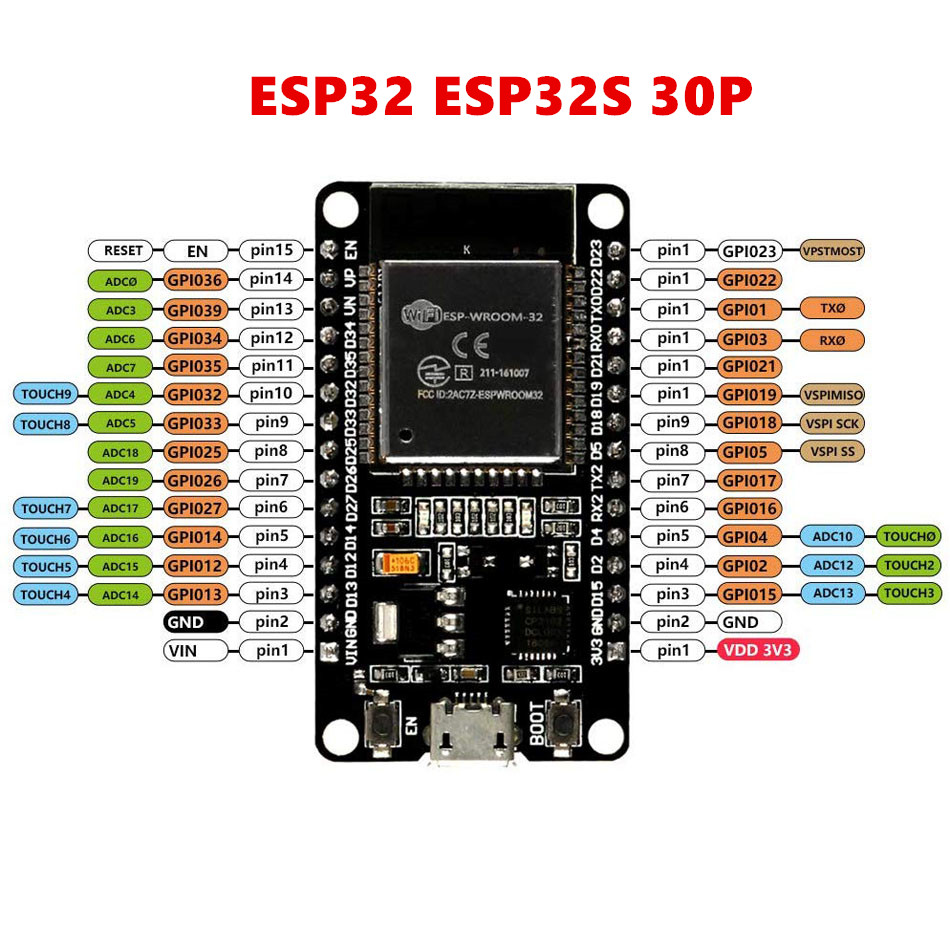
\includegraphics[width=.5\textwidth]{Images/ESP32.jpg}
  \caption{ESP32}
  \label{fig:exampleESP32}
\end{figure}

\subsection{Protoboard}
É uma matriz de matriz de contato, ou contato, ou placa de ensaio (ou em inglês breadboard)
é uma placa com furos de furos de conexões conexões condutoras condutoras para montagem montagem de
circuitos elétricos circuitos elétricos elétricos experimentais experimentais.

\begin{figure}[ht]
  \centering
  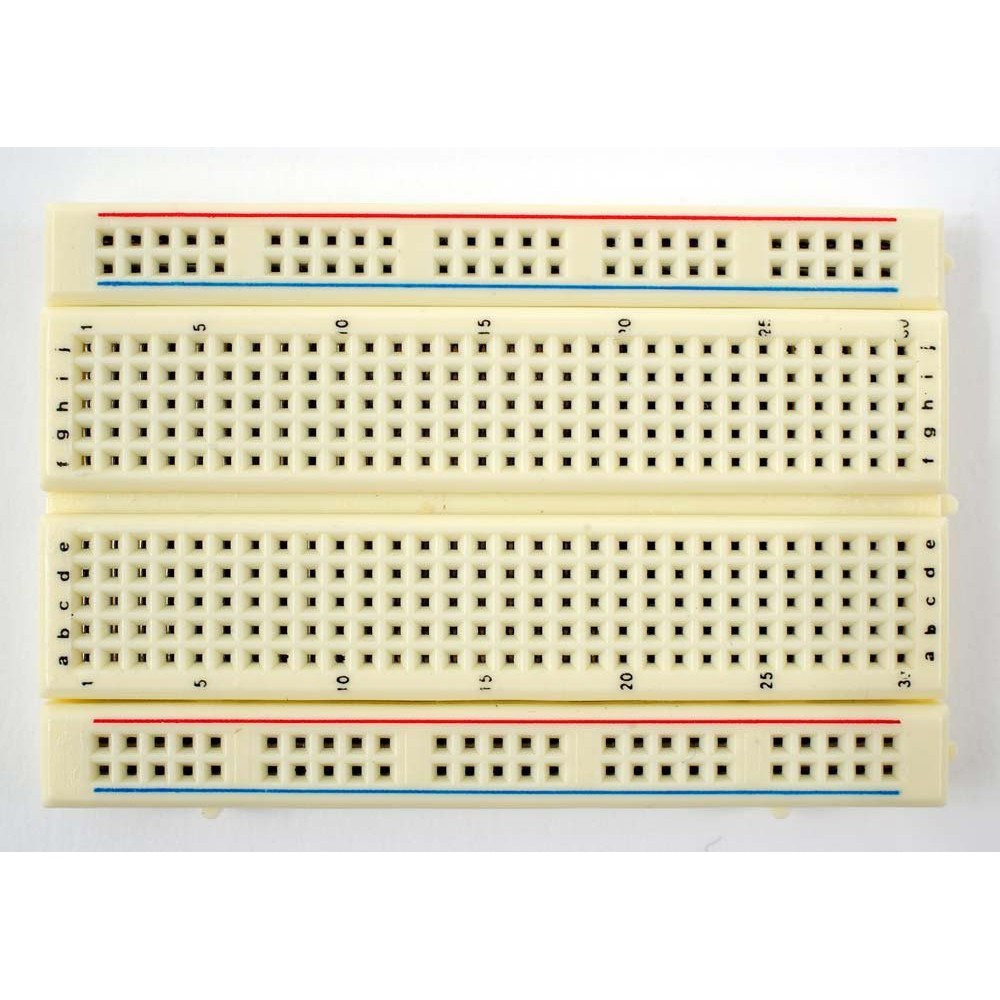
\includegraphics[width=.5\textwidth]{Images/protoboard.jpg}
  \caption{Protoboard}
  \label{fig:exampleProtoboard}
\end{figure}

\subsection{LEDs}
É  um componente eletrônico semicondutor, ou seja, um diodo emissor de luz ( L.E.D = Light emitter diode ),
mesma tecnologia utilizada nos chips dos computadores, que tem a propriedade de transformar energia elétrica em luz.

\begin{figure}[ht]
  \centering
  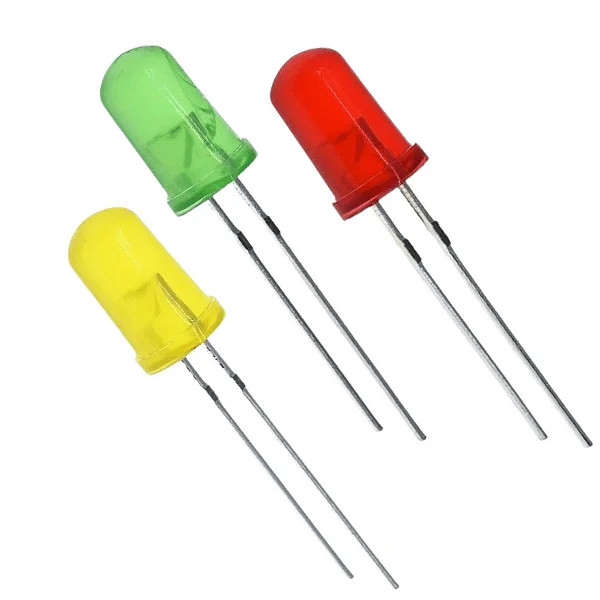
\includegraphics[width=.45\textwidth]{Images/LEDs.jpg}
  \caption{LEDs}
  \label{fig:exampleLEDs}
\end{figure}

\subsection{Jumpers}
São pequenos fios condutores que podem ser conectados a uma protoboard
para interligar dois pontos do circuito em projetos eletrônicos.

\begin{figure}[ht]
  \centering
  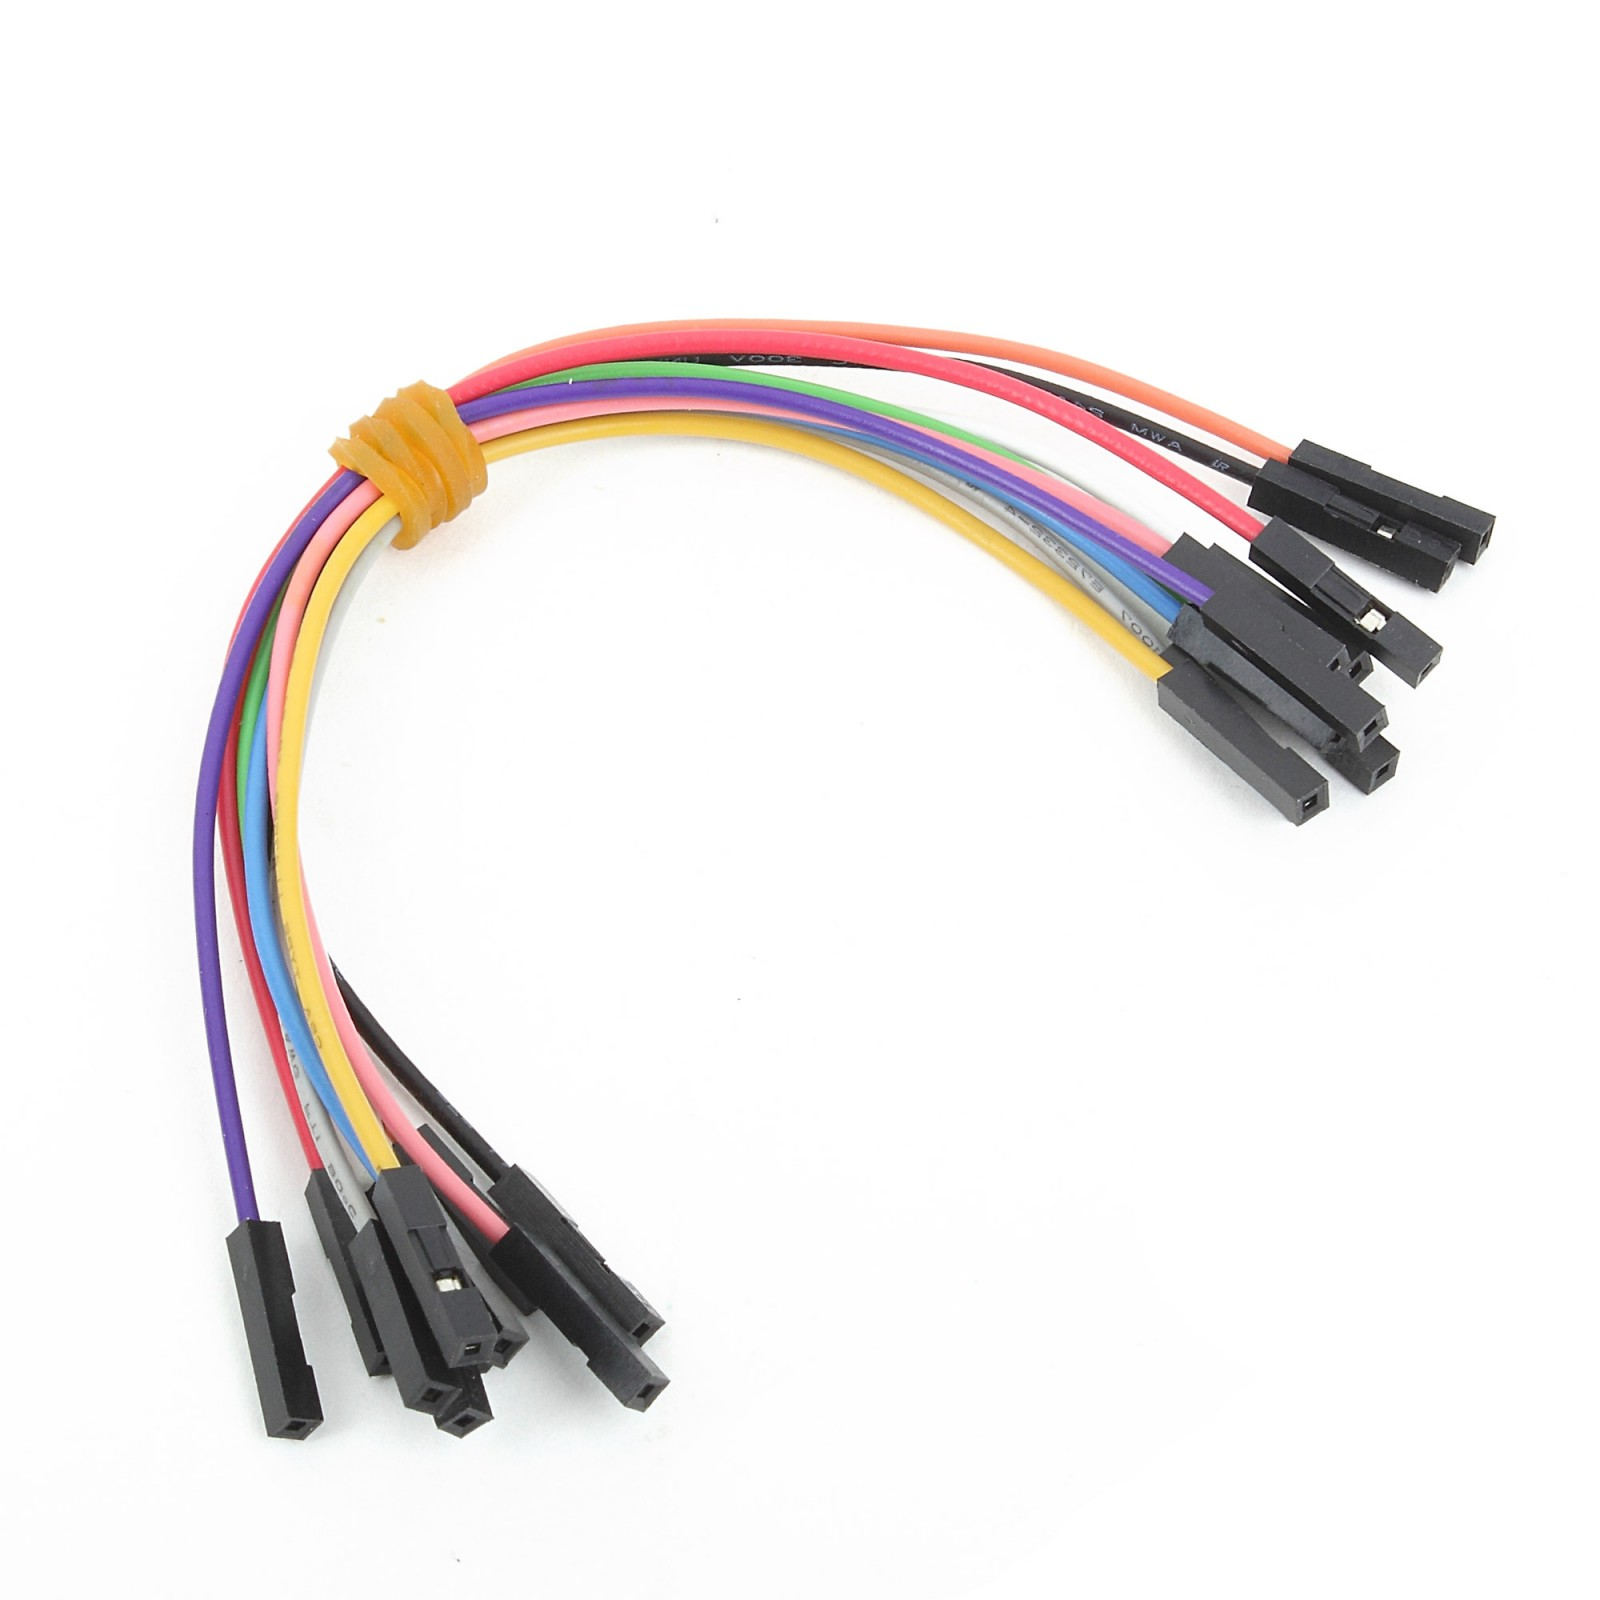
\includegraphics[width=.45\textwidth]{Images/jumpers.jpg}
  \caption{Jumpers}
  \label{fig:exampleJumpers}
\end{figure}
\subsection{ArduinoIDE}
É uma aplicação de plataforma cruzada, escrito em funções de C e C ++. É usado para escrever e fazer upload de
programas em placas compatíveis com Arduino, mas também, com a ajuda de núcleos de terceiros, outras placas de
desenvolvimento de fornecedores.

Para exportar o código para o nosso ESP32 foi adicionado a placa dentro da IDE para que o fosse reconhecido corretamente.

\begin{figure}[ht]
  \centering
  
\includegraphics[width=.45\textwidth]{Images/arduinoIDELogo.png}
  \caption{Logo de ArduinoIDE}
  \label{fig:exampleArduinoIDE}
\end{figure}

\section{Código fonte}
Agora vamos dar uma olhada no código fonte utilizado para passar as instruções para o ESP32
\lstinputlisting[language=C, firstline=1, lastline=29]{code/semafaro.INO}

\section{Resultados}
Juntando tudo oque foi feito conseguimos como resultado o acionamento dos LEDs, com intervalo programado e controlado pelo ESP32.
\begin{figure}[ht]
  \centering
  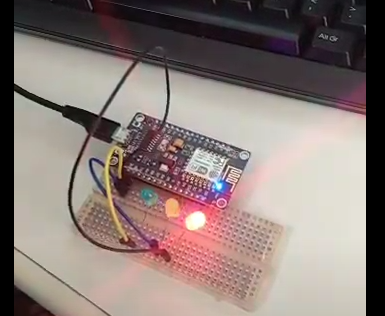
\includegraphics[width=.35\textwidth]{Images/Captura de tela 2022-09-26 140817.png}
  \caption{Resultado}
  \label{fig:exampleLedPiscando}
\end{figure}

O video pode ser acessado clicando em: \emph{\href{https://imgur.com/a/BEnh8kg}{video}}

\bibliographystyle{sbc}
\bibliography{sbc-template}
\nocite{SANDROJUCA}
\end{document}
